
%------------------------------------------------------------------------%
{
\textbf{Uniform Distribution: Example}

\begin{itemize}
\item Suppose there is a platform in a subway station in a large large city. \item Subway trains arrive \textbf{every three minutes} at this platform. \item What is the shortest possible time a passenger would have to wait for a train?
\item What is the longest possible time a passenger will have to wait?
\end{itemize}

}


%------------------------------------------------------------------------%
{
\textbf{Uniform Distribution: Example}

\begin{itemize}
 \item What is the shortest possible time a passenger would have to wait for a train?
%\begin{itemize}
\item If the passenger arrives just before the doors close, then the waiting time is zero.
\[ a = 0 \mbox{ minutes } \]
\end{itemize}
}


%------------------------------------------------------------------------%
{
\textbf{Uniform Distribution: Example}

\begin{itemize}
\item What is the longest possible time a passenger will have to wait?
%\begin{itemize}
\item If the passenger arrives just after the doors close, and missing the train, then he or she will have to wait the full three minutes for the next one.
\[ b = 3 \mbox{ minutes }  = 180 \mbox{ seconds}  \]
\end{itemize}
%\end{itemize}

}

%------------------------------------------------------------------------%
{
\textbf{Uniform Distribution: Example}

\begin{itemize}
\item What is the longest probability that he will have to wait longer than 2 minutes?
\[ P(X \geq 2)  = {3-2 \over 3-0} = {1/3} = 0.33333   \]
\end{itemize}
%\end{itemize}

}

%----------------------------------------------------------------------------------------------------%

\textbf{The Continuous Uniform Distribution}



\begin{center}
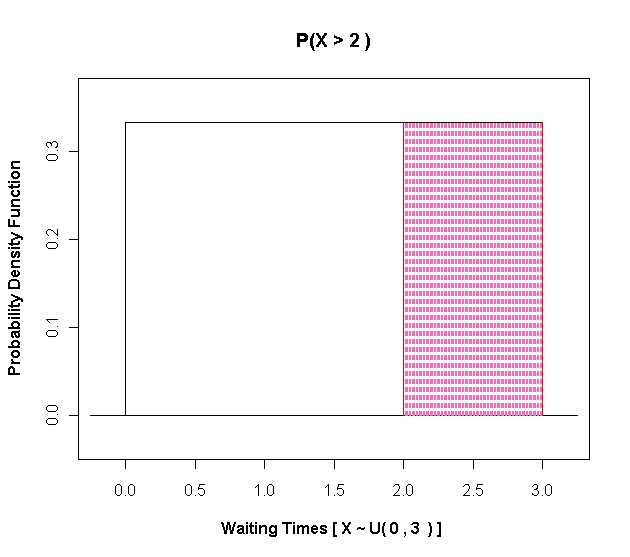
\includegraphics[scale=0.35]{images/6AUniform4}

\end{center}
\medskip
%------------------------------------------------------------------------%
{
\textbf{Uniform Distribution: Example}

\begin{itemize}
\item What is the longest probability that he will have to wait less than than 45 seconds (i.e. 0.75 minutes)?
\[ P(X \leq 0.75)  = {0.75 - 0 \over 3-0} = {0.75/3} = 0.250  \]
\end{itemize}
%\end{itemize}

}



%----------------------------------------------------------------------------------------------------%

\textbf{The Continuous Uniform Distribution}



\begin{center}
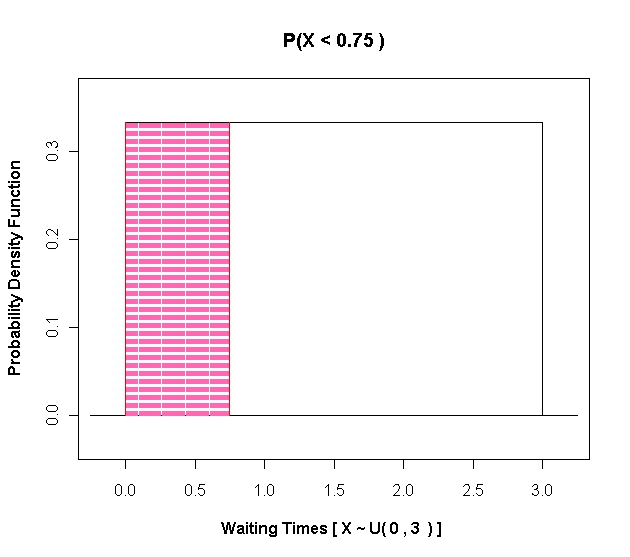
\includegraphics[scale=0.35]{images/6AUniform3}

\end{center}
\medskip
%------------------------------------------------------------------------%
{
\textbf{Uniform Distribution: Expected Value}

We are told that, for waiting times,  the lower limit $a$ is 0, and the upper limit $b$ is 3 minutes. \\ \bigskip The expected waiting time $\textrm{E}[X]$ is computed as follows
\vspace{0.1cm}
\[
\textrm{E}[X] = {b + a \over 2} =  {3 + 0  \over 2}  = 1.5 \mbox{ minutes }
\]

}
%------------------------------------------------------------------------%
{\textbf{Uniform Distribution: Variance}

The variance of the continuous uniform distribution, denoted $\textrm{V}[X]$,  is  computed using the following formula
\vspace{0.1cm}
\[
\textrm{V}[X] = {(b - a)^2 \over 12}
\]
\vspace{0.1cm}
For our previous example this is
\[
\textrm{V}[X] = {(3 - 0)^2 \over 12} =  {3^2 \over 12} = {9 \over 12} = 0.75
\]
}

